%Use 16:9
\documentclass[dvipsnames]{beamer}
\usepackage{graphicx} % Required for inserting images
\usepackage{xcolor}
\definecolor{codebg}{HTML}{0D1117} % GitHub Dark background
\usepackage[newfloat]{minted}
\usepackage{fontspec}
\setmonofont{Fira Code}
% Colors
\usepackage{xcolor}

% Use the same style everywhere
\usemintedstyle{monokai}

% Global minted defaults (including background)
\setminted{
  breaklines,
  breakanywhere,
  linenos,
  numbersep=6pt,
  fontsize=\footnotesize,
  xleftmargin=1em,
  tabsize=2,
  bgcolor=codebg,             % <<< make minted's background dark
}

% C++-specific tweaks
\setminted[c++]{
  mathescape,
  escapeinside=||,
}


% Make line numbers readable on dark bg (optional but nice)
\makeatletter
\renewcommand\theFancyVerbLine{%
  \textcolor{white!60}{\arabic{FancyVerbLine}}%
}
\makeatother

% tcolorbox wrapper: use the same background + a subtle frame
\usepackage[most]{tcolorbox}
\tcbuselibrary{minted,skins,breakable}
\newtcblisting{cppcode}[1][]{
  listing engine=minted,
  minted language=c++,
  minted style=monokai,  % keep in sync
  minted options={
    linenos,autogobble,breaklines,fontsize=\footnotesize,
    mathescape,escapeinside=||,
 %   bgcolor=codebg,          % <<< align inner bg with the box
  },
%  colback=codebg,            % <<< box background
  colframe=white!10,         % subtle border against black
  enhanced, breakable,
  boxrule=0.4pt, arc=2.5pt,
  left=1em, right=1em, top=0.6em, bottom=0.6em,
  borderline west={2.2pt}{0pt}{blue!65!black}, % accent stripe
  #1
}
\usepackage{mathtools}
\usepackage[thinc]{esdiff}
\usepackage{tikz}
\usetikzlibrary{shapes,arrows,positioning}
\usetikzlibrary{calc}
\usepackage{listings}
\usepackage{tikz}
\usetikzlibrary{shapes, arrows.meta, positioning}
\usepackage{animate}
% --- Minimal 64B cache line utilities ---------------------------------------
% Requires: \usepackage{tikz} \usetikzlibrary{arrows.meta}
% Environment draws an 8-block bar; you add colors/marks inside it.
\newenvironment{CacheLine}[1][]{
  \begin{tikzpicture}[x=1.2cm,y=0.8cm,font=\footnotesize,>=Stealth,#1]
    % Geometry knobs (in "y units"); tweak with \CacheSetBelow if needed.
    \def\CacheH{1.0}   % bar height
    \def\CacheBelow{1.0} % how far below the bar the bottom labels sit

    % (We fill blocks and draw marks here; lines/labels go at the end)
}{
    % Vertical dividers and labels (drawn last so they sit on top of fills)
    \foreach \i in {1,...,7} { \draw[black!40] (\i,0) -- (\i,\CacheH); }
    \draw[line width=0.6pt, rounded corners=2pt] (0,0) rectangle (8,\CacheH);
    \foreach \i in {0,...,7} {
      \node[below=3pt, text=black!75] at (\i+0.5,0) {8B \i};
    }
  \end{tikzpicture}
}

% Color a single 8B block i with a given color (keeps lines visible via opacity)
% Usage: \CacheColor{<i 0..7>}{<color>}
\newcommand{\CacheColor}[2]{%
  \fill[#2, fill opacity=0.35, draw=none] (#1,0) rectangle ++(1,\CacheH);%
}

% Color a contiguous range of blocks [i,j) (e.g., 2..5 colors blocks 2,3,4)
% Usage: \CacheColorRange{<i>}{<j>}{<color>}
\newcommand{\CacheColorRange}[3]{%
  \fill[#3, fill opacity=0.35, draw=none] (#1,0) rectangle (#2,\CacheH);%
}

% Mark the START (left edge) of block i with an arrow and label ABOVE.
% Usage: \CacheMarkAbove[<color>]{<i 0..7>}{<label>}
\newcommand{\CacheMarkAbove}[3][green!60!black]{%
  \draw[-{Stealth[length=3mm]}, very thick, draw=#1] (#2,\CacheH+0.36) -- (#2,\CacheH+0.04);
  \node[above, text=#1] at (#2,\CacheH+0.36) {#3};
}

% Mark the START (left edge) of block i with an arrow and label BELOW.
% (Moved further down so it clears the "8B k" tick labels.)
% Usage: \CacheMarkBelow[<color>]{<i 0..7>}{<label>}
\newcommand{\CacheMarkBelow}[3][green!60!black]{%
  \draw[-{Stealth[length=3mm]}, very thick, draw=#1] (#2,-\CacheBelow+0.28) -- (#2,0.02);
  \node[below, anchor=west, text=#1] at (#2,-\CacheBelow-0.2) {#3};
}

% Optional: adjust how far below the bar the bottom labels/arrows go (in "y units")
% e.g., \CacheSetBelow{1.2} pushes them farther down.
\newcommand{\CacheSetBelow}[1]{\def\CacheBelow{#1}}
% ---------------------------------------------------------------------------

\title{Reverse Mode Automatic Differentiation: Unraveling Expression Graphs \& Library Magic}
\author{Steve Bronder}
\date{October 2023}

\def\mathcolor#1#{\@mathcolor{#1}}
\def\@mathcolor#1#2#3{%
  \protect\leavevmode
  \begingroup
    \color#1{#2}#3%
  \endgroup
}

\newcommand{\fracp}[2]{\frac{\partial #1}{\partial #2}}
\newcommand{\pp}[2]{\frac{\partial#1}{\partial#2}}
\newcommand{\adj}[1]{\bar{#1}}
\newcommand{\pluseq}{\mathrel{+}=}

\makeatother

\addtobeamertemplate{navigation symbols}{}{%
    \usebeamerfont{footline}%
    \usebeamercolor[fg]{footline}%
    \hspace{1em}%
    \insertframenumber/\inserttotalframenumber
}

\begin{document}
\expandafter\def\expandafter\insertshorttitle\expandafter{%
  \insertshorttitle\hfill%
  \insertframenumber\,/\,\inserttotalframenumber}
\maketitle
% Slide

\begin{comment}

{ % all template changes are local to this group.
    \setbeamertemplate{navigation symbols}{}
    \begin{frame}<article:0>[plain]
        \begin{tikzpicture}[remember picture,overlay]
            \node[at=(current page.center)] {
                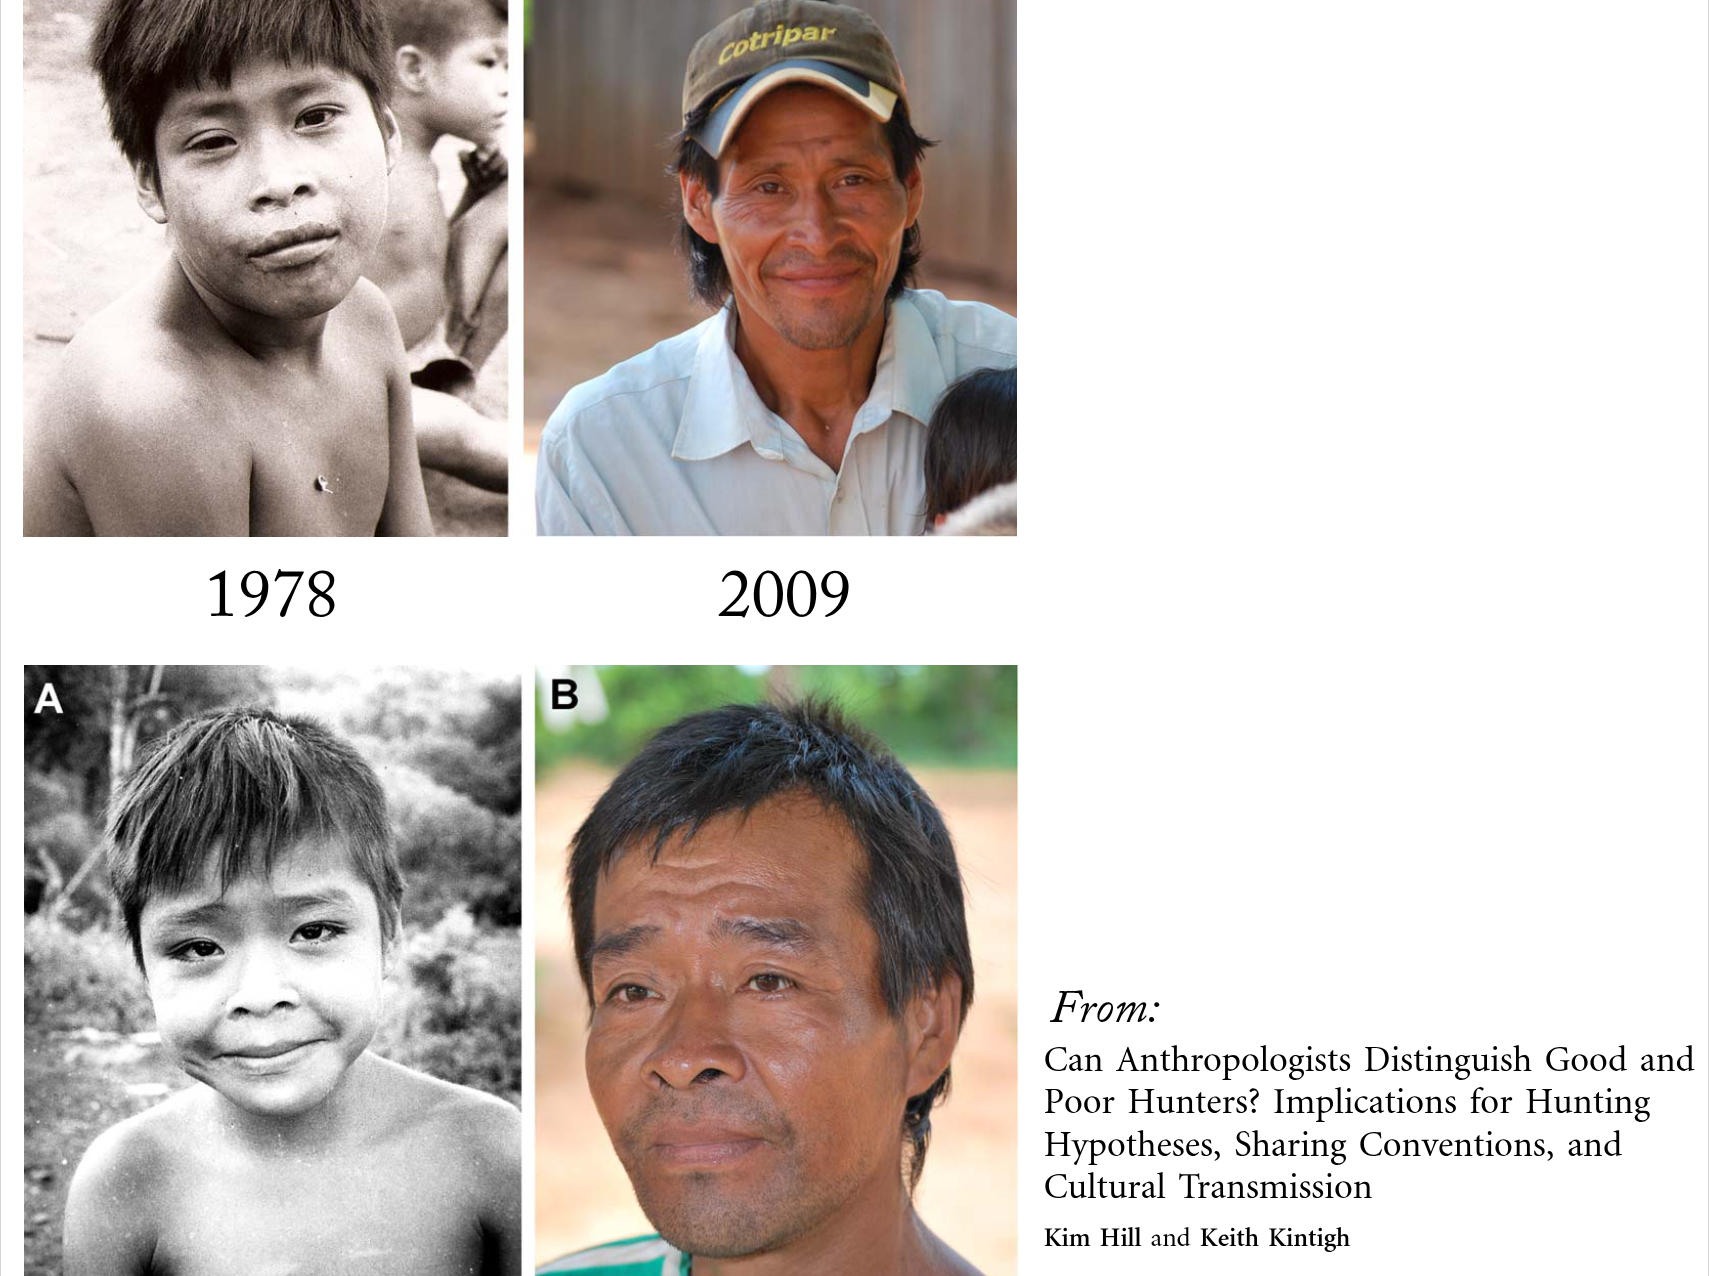
\includegraphics[keepaspectratio,
                                 width=\paperwidth,
                                 height=\paperheight]{img/mcel1.png}
            };
        \end{tikzpicture}
     \end{frame}
}

{ % all template changes are local to this group.
    \setbeamertemplate{navigation symbols}{}
    \begin{frame}<article:0>[plain]
        \begin{tikzpicture}[remember picture,overlay]
            \node[at=(current page.center)] {
                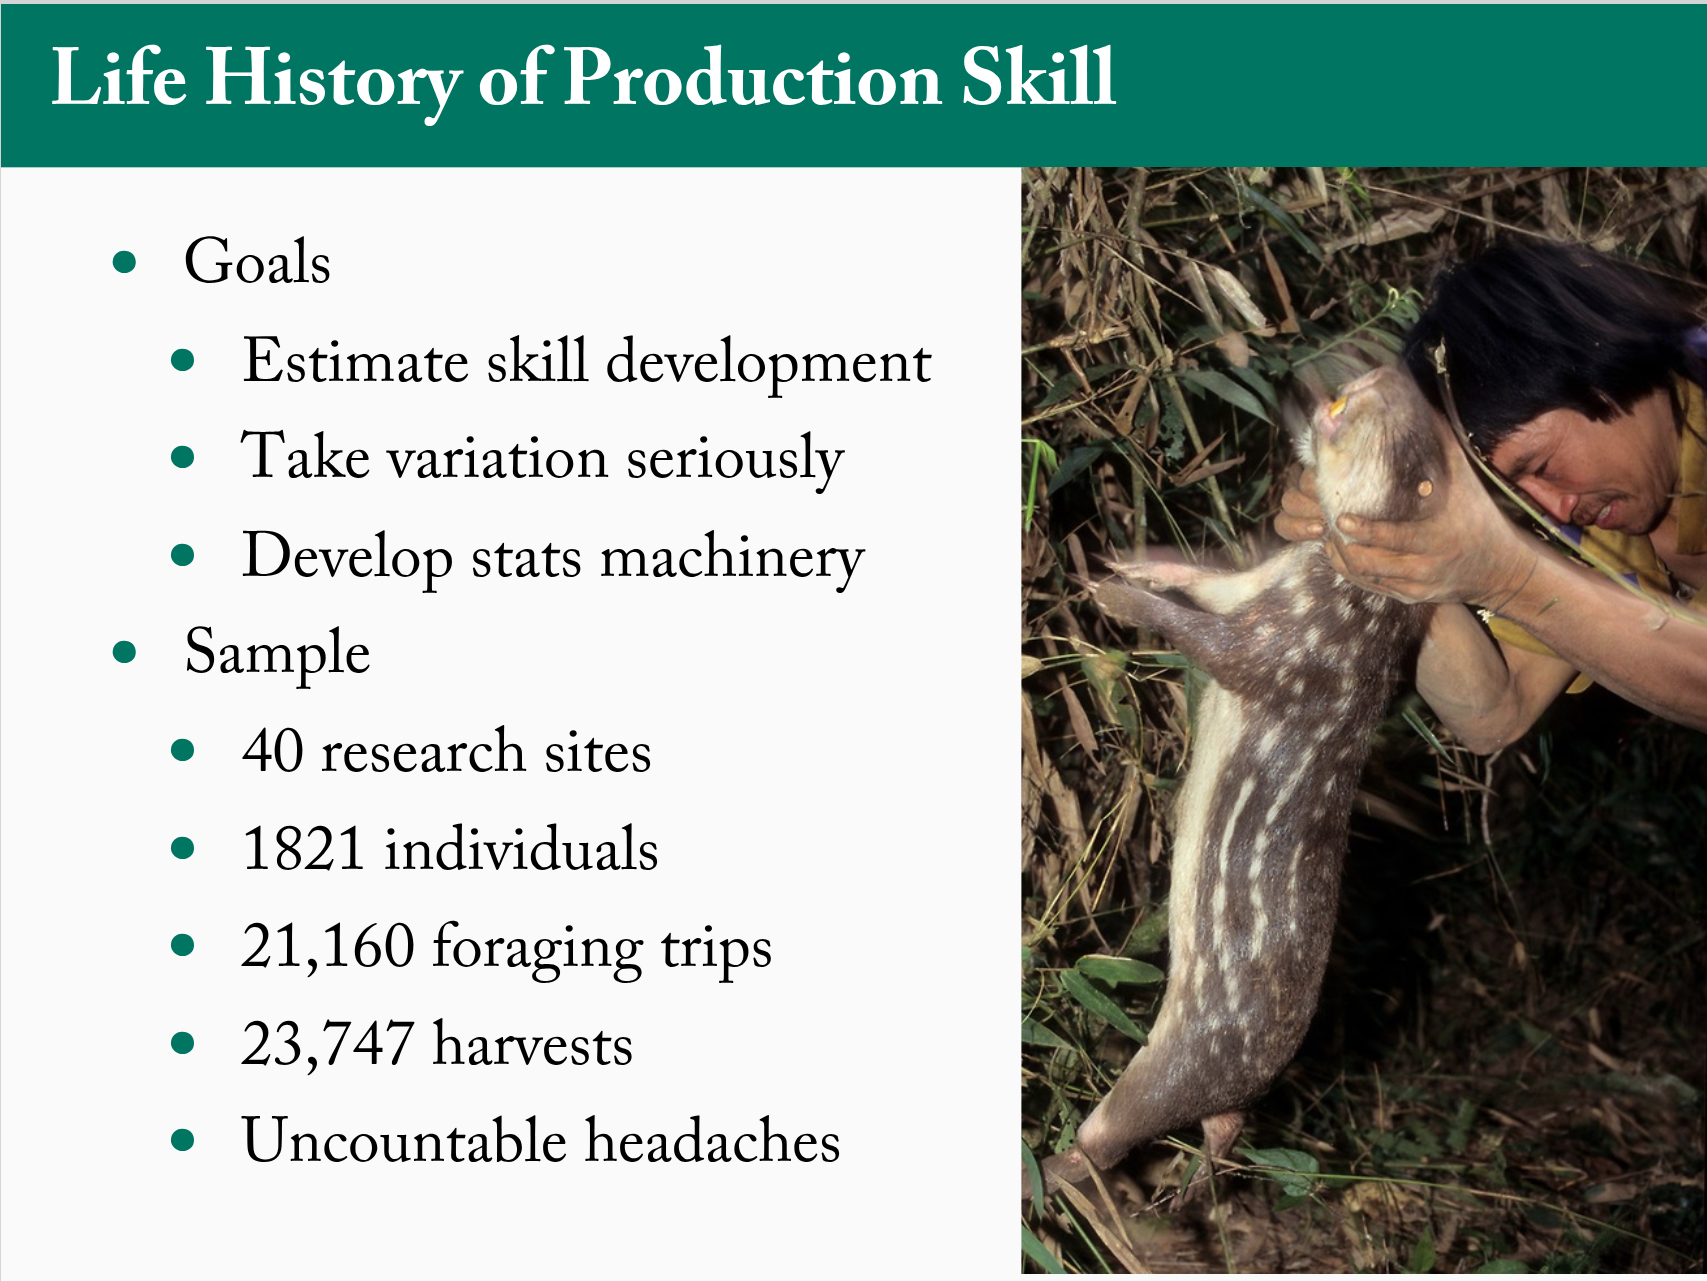
\includegraphics[keepaspectratio,
                                 width=\paperwidth,
                                 height=\paperheight]{img/mcel2.png}
            };
        \end{tikzpicture}
     \end{frame}
}

{ % all template changes are local to this group.
    \setbeamertemplate{navigation symbols}{}
    \begin{frame}<article:0>[plain]
        \begin{tikzpicture}[remember picture,overlay]
            \node[at=(current page.center)] {
                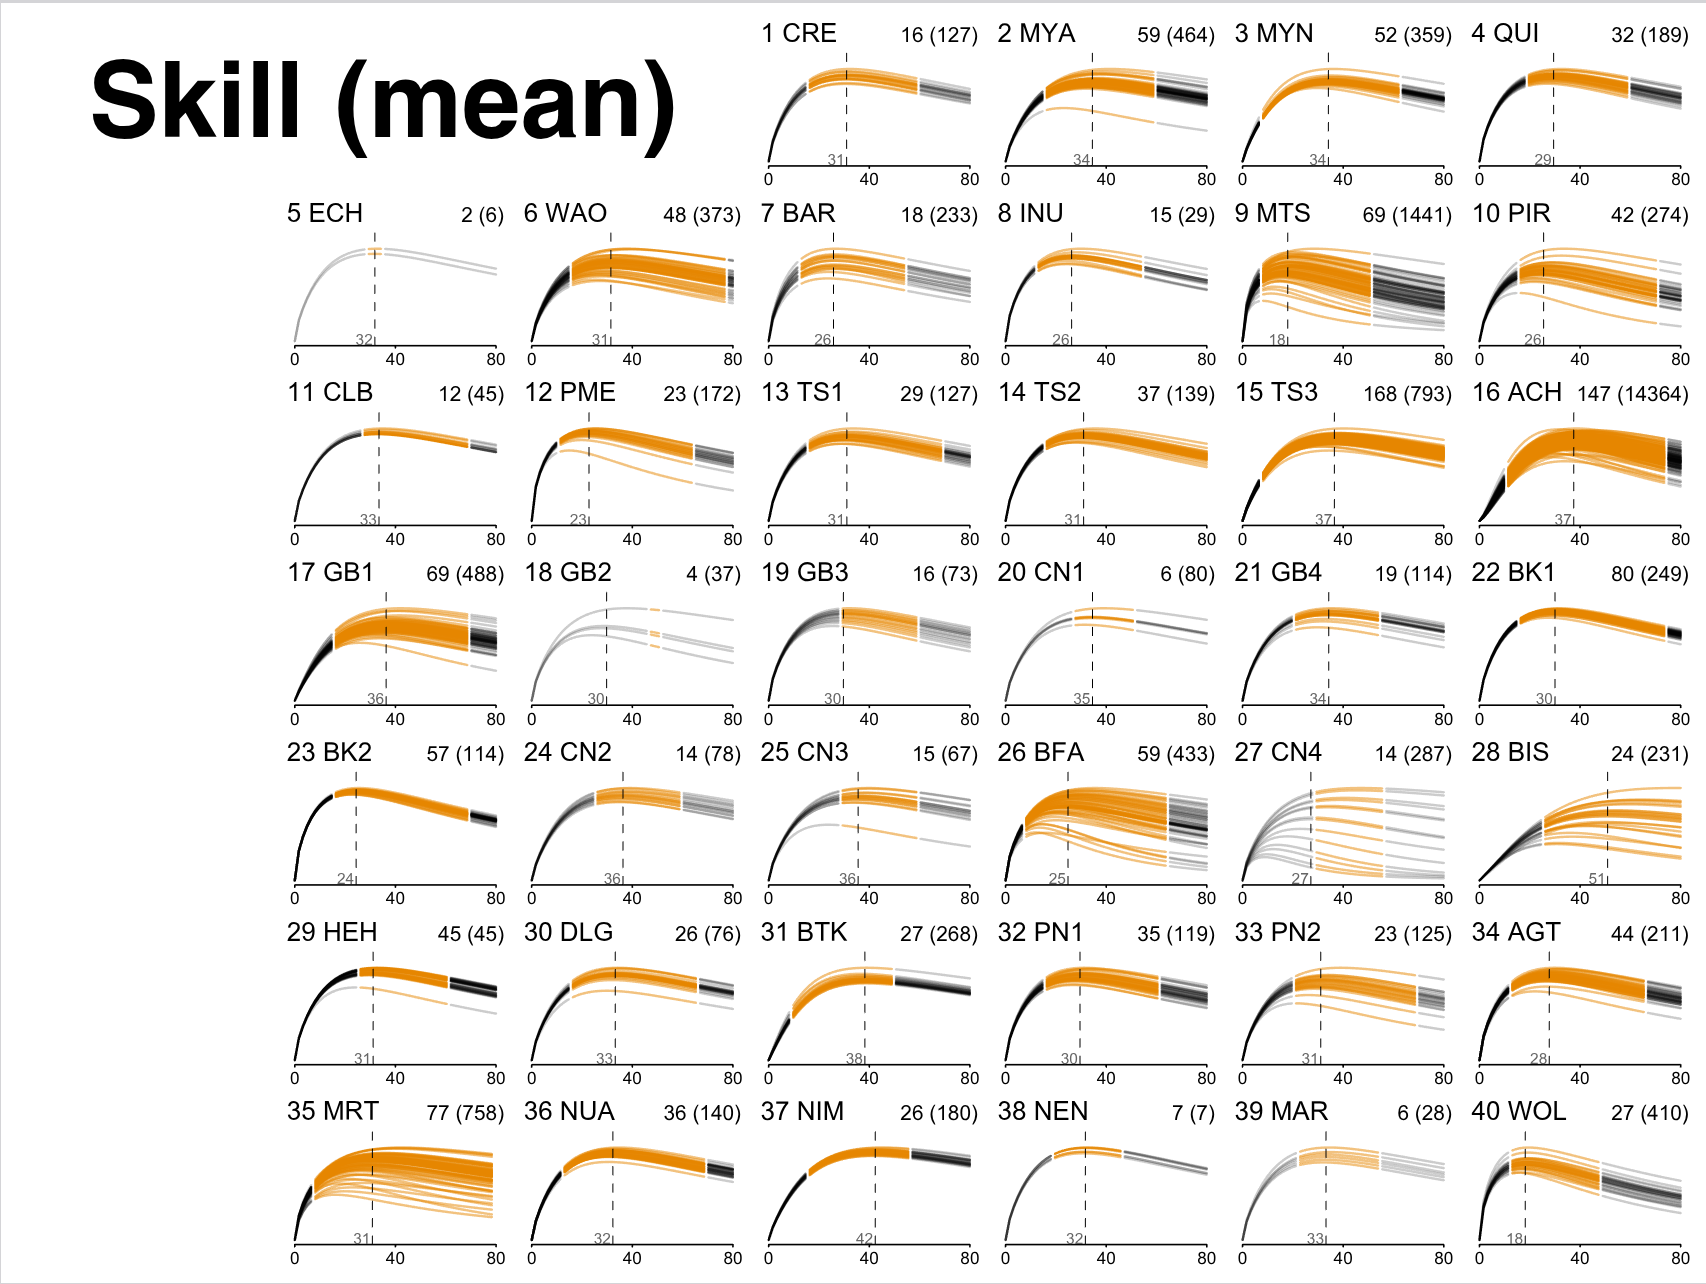
\includegraphics[keepaspectratio,
                                 width=\paperwidth,
                                 height=\paperheight]{img/mcel3.png}
            };
        \end{tikzpicture}
     \end{frame}
}
\end{comment}
\begin{frame}{Estimating COVID Infection Rates For Policy}
\begin{figure}
\centerline{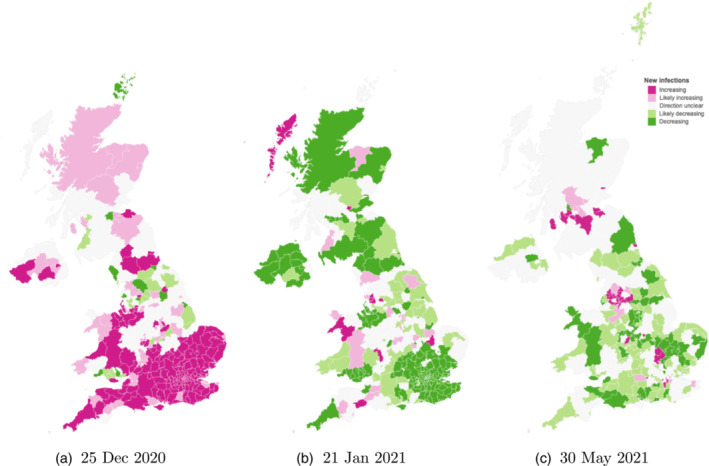
\includegraphics[scale=.5]{img/covid_uk.jpg}}
\caption{Probability of epidemic growth by local area}
\label{fig-covid}
\end{figure}
\end{frame}

\note{These models can only exist because autodiff exists}
\begin{frame}{Automatic Differentiation  Affects Your Day to Day}
\begin{figure}
\centerline{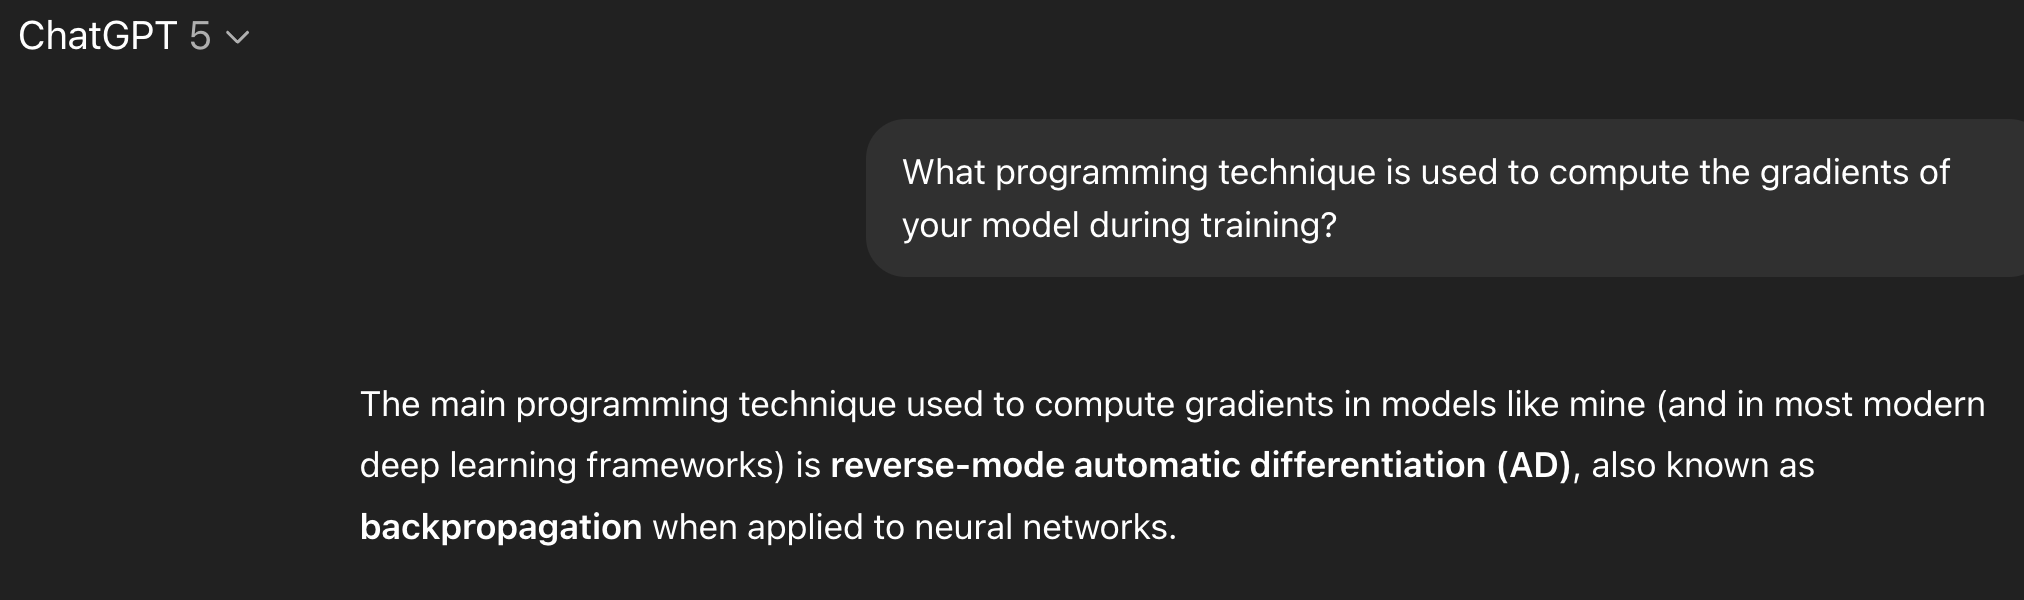
\includegraphics[scale=.16]{img/chatgpt.png}}
\label{fig-chatgpt}
\end{figure}
\end{frame}

\note{Autodiff is the mitochondria of machine learning. AD allows for efficient estimation of many statistical models.}

\begin{frame}{What is Automatic Differentiation?}
Computational technique for evaluating derivatives of functions expressed as computer programs by systematically applying the chain rule.
\end{frame}

\begin{frame}{Why use Automatic Differentiation}
Ex: Newton's root finding method
\begin{equation*}
    x_{n+1} = x_n - \frac{f\left(x_n\right)}{f\,'\left(x_{n}\right)}
\end{equation*}
find $f(x)=y$ where $y=0$
\end{frame}
\note{
How do we estimate solutions for equations? A simple method is the newton method.
Why are gradients useful? We use gradients to solve
For models we want to estimate parameter values. Change the slide here so that we show how to solve for parameters using newtons method
}

\begin{frame}{Why use Automatic Differentiation?}
\begin{align}
    f(x) &= x^3 + x^2 + x\\
    f\,'(x) &= 3x^2 + 2x + 1
\end{align}
\centering
\animategraphics[loop,controls,scale=0.35]{2}{gif/newton-}{0}{17}
\end{frame}

\begin{frame}{Why use Automatic Differentiation?}
\begin{itemize}
    \item Hamiltonian Monte Carlo:
    \begin{itemize}
    \item $\frac{dp}{dt}=-\nabla_\theta\log p(\theta|y)$
    \end{itemize}
    \item BFGS:
    \begin{itemize}
    \item $s_k=-H_k \nabla_\theta f(\theta_k)$
    \end{itemize}
    \item Stochastic Gradient Descent:
    \begin{itemize}
    \item $\theta_{t+1}=\theta_t−\eta\nabla_\theta L(\theta_t;x_t)$
    \end{itemize}
\end{itemize}
\end{frame}

\begin{frame}{Why use Automatic Differentiation?}
\begin{itemize}
    \item Choices
    \begin{itemize}
        \item Write by hand
        \item finite difference,
        \item symbolic differentiation
        \item spectral differentiation
        \item automatic differentiation
    \end{itemize}
\end{itemize}
\end{frame}


\begin{frame}{Why use Automatic Differentiation?}

\tiny
\begin{align*}
&\underbrace{p\!\left(
\boldsymbol{\theta} \,\big|\, \mathbf y
\right)}_{\textbf{posterior}}
\;\propto\;
\prod_{i=1}^{N}
\Bigg\{
\sum_{\mathbf z_i \in \{1,2,3\}^{T_i}}
\!\Bigg[
\underbrace{\pi_{z_{i,1}}\prod_{t=2}^{T_i}\Pi_{z_{i,t-1},\,z_{i,t}}}_{\text{3-state HMM prior}}
\;
\prod_{t=1}^{T_i}
\underbrace{\mathcal N\!\Big(
y_{i,t}\,\Big|\,\eta_{i,t},\,\sigma_{z_{i,t}}^{2}
\Big)}_{\text{state-dependent emission}}
\Bigg]
\Bigg\}
\\[-2pt]
&\text{where}\quad
\eta_{i,t}
=\underbrace{\mathbf x_{i,t}^{\!\top}\boldsymbol\beta}_{\text{fixed}}
+\underbrace{\mathbf z^{(G)}_{i,t}{}^{\!\top}\mathbf b_{g[i]}
+\mathbf z^{(C)}_{i,t}{}^{\!\top}\mathbf c_{c[i]}
+u_{g[i]}}_{\text{crossed random effects}}
+\underbrace{f(t_{i,t})}_{\text{GP}}
+\underbrace{\mu_{z_{i,t}}
+\mathbf r_{z_{i,t}}^{\!\top}\mathbf w_i}_{\text{state-specific offset + slope}}
,\qquad z_{i,t}\in\{1,2,3\}.
\\[4pt]
&
p(\mathbf f\mid\boldsymbol\psi)
=
(2\pi)^{-T/2}\,|\mathbf K|^{-1/2}\;
\exp\!\Big(-\tfrac12\,\mathbf f^{\!\top}\mathbf K^{-1}\mathbf f\Big),
\\[-2pt]
&
\mathbf K
=\sigma_f^{2}\Big(\mathbf K_{\text{LP}}(\ell,p,\lambda)\;+\;\rho\,\mathbf K_{\text{SE}}(\tilde\ell)\Big)
+\sigma_n^{2}\mathbf I,\quad
\big[\mathbf K_{\text{LP}}\big]_{t t\,'}
=\exp\!\left(
-\frac{(t-t')^{2}}{2\ell^{2}}
-\frac{2\sin^{2}\!\big(\pi|t-t'|/p\big)}{\lambda^{2}}
\right),
\\[-2pt]
&
\big[\mathbf K_{\text{SE}}\big]_{t t'}
=
\exp\!\left(-\frac{(t-t')^{2}}{2\tilde\ell^{2}}\right),
\qquad
\mathbf K=\mathbf L_K\mathbf L_K^{\!\top}
\;\Rightarrow\;
\log|\mathbf K|=2\sum_{j=1}^{T}\log \big((\mathbf L_K)_{jj}\big).
\\[6pt]
&\textbf{Hierarchical mixed effects (non-centered, LKJ prior):}
\\[-2pt]
&\qquad
\mathbf b_{g}=\big(\mathbf I_{p_G}\otimes\operatorname{diag}(\boldsymbol\tau_b)\,\mathbf L_R\big)\,\tilde{\mathbf b}_{g},
\;\;
\tilde{\mathbf b}_{g}\sim\mathcal N(\mathbf 0,\mathbf I),
\;\;
\mathbf c_{c}=\operatorname{diag}(\boldsymbol\tau_c)\,\tilde{\mathbf c}_{c},
\;\;
\tilde{\mathbf c}_{c}\sim\mathcal N(\mathbf 0,\mathbf I),
\\[-2pt]
&\qquad
\operatorname{LKJ}_{p_G}(\eta)\ \text{prior on}\ \mathbf R,\quad
\mathbf L_R\mathbf L_R^{\!\top}=\mathbf R,
\quad
\boldsymbol\tau_b\sim\prod_{j=1}^{p_G}\text{Half-}t_{\nu_b}(0,s_b),
\quad
\boldsymbol\tau_c\sim\prod_{j=1}^{p_C}\text{Half-}t_{\nu_c}(0,s_c),
\\[-2pt]
&\qquad
u_g\sim\mathcal N(0,\sigma_u^2).
\end{align*}


\end{frame}
\begin{frame}{Why use Automatic Differentiation?}
\begin{itemize}
\item Faster than finite difference, more flexible than symbolic differentiation
\item Allows for unknown length while and for loops
\item Accurate to floating point precision
\item Reverse Mode AD can compute partials derivatives of inputs at the same time
\end{itemize}
\end{frame}

\begin{frame}{How Fast is AutoDiff?}
\begin{figure}
\centerline{
\includegraphics[scale=.5]{img/mocking-spongebob.jpg}}
\caption{AuToDiFf rUnS iN $\Theta(C(f))$ TiMe}
\label{fig-spongebob}
\end{figure}
\end{frame}

\begin{frame}{Implementation Matters!}
\begin{figure}
\centerline{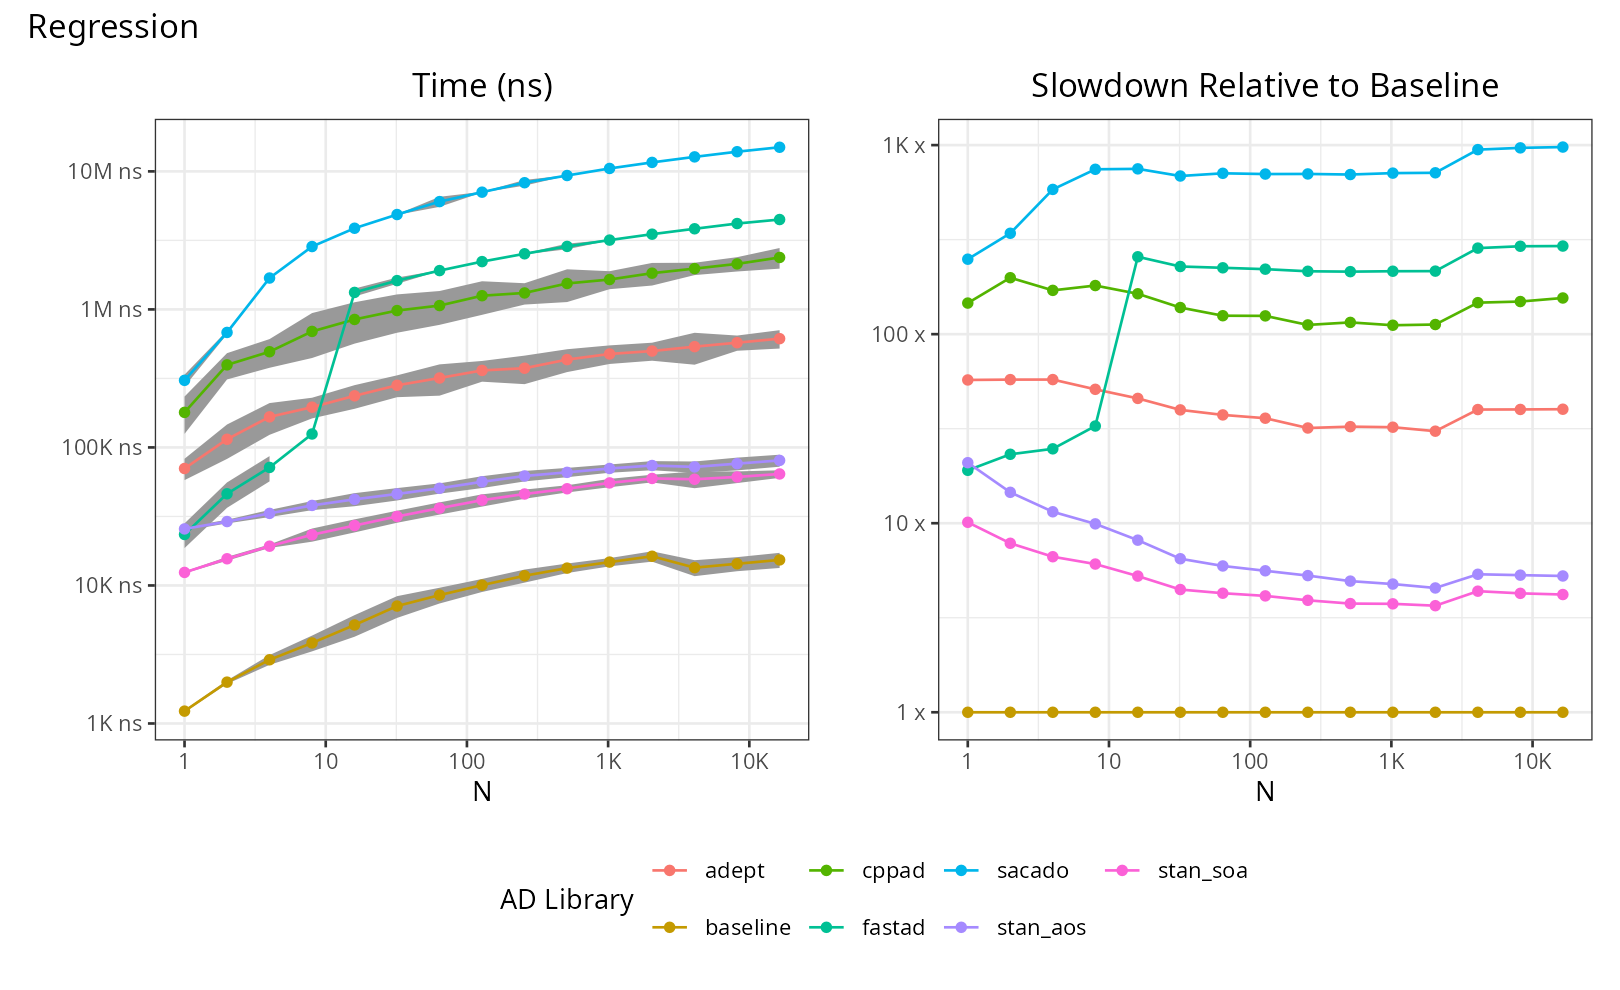
\includegraphics[scale=.5]{img/combined_regression_plot.png}}
\caption{Benchmark for $f\,'$ given $f(y) = N(y | X\theta,\sigma)$}
\label{fig-red-bench}
\end{figure}
\end{frame}

\begin{frame}{Goal of this talk}
\begin{itemize}
    \item Explain autodiff in layman's terms
    \item Understand performance of high throughput memory intensive programs
    \item Show how modern C++ has led to cleaner and more efficient AD
\end{itemize}
\end{frame}

\note{Let $v_k$ be the sequence of intermediate expressions for the input $x$ and output $z$ and let $v_K = z$ and $v_0 = x; v_1 = y$. Let $\overline{v}_k$ be the partial gradient of the kth intermediate step. Then we can apply the chain rule to each intermediate step to get the partial gradient.
}

\begin{frame}[fragile]{What is Automatic Differentiation?}
\begin{itemize}
  \item AD computes gradients of a program by applying the chain rule to its subexpressions.
  \item Given a function $f$ with inputs $x\in\mathbb{R}^n$ and outputs $z\in \mathbb{R}^m$ we want to "calculate the Jacobian $J\,$" with size $(m, n)$
\end{itemize}
%Automatic Differentiation can do higher order partials, but here we just focus on the first order
\end{frame}

\note{Emphasize: AD is mechanical chain rule over the executed program, not symbolic math or numeric differencing.}

\begin{frame}{Data Type: Expression Graph}
Goal: Calculate the full gradient by accumulating partial gradients (adjoints) through the a graph of subexpressions.

 \begin{itemize}
%     \item Dependency graph of intermediate computations
     \item Think of both data and operations as objects
     \begin{itemize}
     \item Forward pass to calculate the values of the intermediates subexpressions
     \item Reverse pass to calculate the local adjoint-Jacobian update of subexpressions
     \end{itemize}
 \end{itemize}
 \end{frame}

\begin{frame}{What is Automatic Differentiation}
 For Reverse Mode AD, each node performs two functions.
\begin{itemize}
 \item Forward Pass:
 \begin{equation*}
     u = f(x, y)
 \end{equation*}
 \item Reverse Pass: Given $u$'s adjoint (partial gradient) $\overline{u}$
 \\Calculate the local adjoint-Jacobian update for $x$ and $y$.
 \begin{equation*}
 chain(\overline{u}, x, x_{1}) = \left\{\overline{x} \pluseq \diffp{u}{{x}}\overline{u},\overline{y} \pluseq \diffp{u}{{y}}\overline{u}\right\}
 \end{equation*}
 \item The calculations needed are represented as an expression Graph
\end{itemize}
\end{frame}

% Slide 1
\begin{frame}{Forward Pass}
\vspace{-1mm}
$$z = \log(x*y)$$

\begin{tikzpicture}
  [
    Round/.style={circle, draw=black!, fill=green!0, thick, minimum size=2mm},
    Red/.style={circle, draw=black!, fill=red!255, thick, minimum size=2mm},
    Yellow/.style={circle, draw=black!, fill=yellow!255, thick, minimum size=10mm},
    Gray/.style={circle, draw=black!, fill=gray!35, thick, minimum size=2mm}
  ]
  % Nodes
  \node[Gray] (v0) at(-8, 0) {$y$};

  \node[Gray] (v1) at(0, 0) {$x$};

  \node[Round] (v2) at(-4, -2) {$*$};

  \node[Round] (v3) at(-6, -4) {$\log$};



  % Lines
  \path [<-, draw, thick] (v2) -- (v0);
  \path [<-, draw, thick] (v2) -- (v1);
  \path [<-, draw, thick] (v3) -- (v2);

\end{tikzpicture}
\end{frame}

\begin{frame}{Forward Pass}
\vspace{-1mm}
$$z = \log(\mathcolor{red}{x} \cdot \mathcolor{red}{y})$$

\begin{tikzpicture}
  [
    Round/.style={circle, draw=black!, fill=green!0, thick, minimum size=2mm},
    Red/.style={circle, draw=black!, fill=red!255, thick, minimum size=2mm},
    Yellow/.style={circle, draw=black!, fill=yellow!255, thick, minimum size=10mm},
    Gray/.style={circle, draw=black!, fill=gray!35, thick, minimum size=2mm}
  ]
  % Nodes
  \node[Gray, label=left:{\textcolor{blue}{$v_0$}}] (v0) at(-8, 0) {$\mathcolor{red}{y}$};

  \node[Gray, label=left:{\textcolor{blue}{$v_1$}}] (v1) at(0, 0) {$\mathcolor{red}{x}$};

\end{tikzpicture}
\end{frame}

\begin{frame}{Forward Pass}
\vspace{-1mm}
$$z = \log(x\mathcolor{red}{\cdot}y)$$

\begin{tikzpicture}
  [
    Round/.style={circle, draw=black!, fill=green!0, thick, minimum size=2mm},
    Red/.style={circle, draw=black!, fill=red!255, thick, minimum size=2mm},
    Yellow/.style={circle, draw=black!, fill=yellow!255, thick, minimum size=10mm},
    Gray/.style={circle, draw=black!, fill=gray!35, thick, minimum size=2mm}
  ]
  % Nodes
  \node[Gray, label=left:{\textcolor{blue}{$v_0$}}] (v0) at(-8, 0) {$y$};

  \node[Gray, label=left:{\textcolor{blue}{$v_1$}}] (v1) at(0, 0) {$x$};

  \node[Round, label=left:{\textcolor{blue}{$v_2 = v_0 \cdot v_1$}}] (v2) at(-4, -2) {$\mathcolor{red}{\cdot}$};


  % Lines
  \path [<-, draw, thick] (v2) -- (v0);
  \path [<-, draw, thick] (v2) -- (v1);

\end{tikzpicture}
\end{frame}

\begin{frame}{Forward Pass}
\vspace{-1mm}
$$z = \mathcolor{red}{\log}(x\cdot y)$$
\begin{tikzpicture}
  [
    Round/.style={circle, draw=black!, fill=green!0, thick, minimum size=2mm},
    Red/.style={circle, draw=black!, fill=red!255, thick, minimum size=2mm},
    Yellow/.style={circle, draw=black!, fill=yellow!255, thick, minimum size=10mm},
    Gray/.style={circle, draw=black!, fill=gray!35, thick, minimum size=2mm}
  ]
  % Nodes
  \node[Gray, label=left:{\textcolor{blue}{$v_0$}}] (v0) at(-8, 0) {$y$};
  \node[Gray, label=left:{\textcolor{blue}{$v_1$}}] (v1) at(0, 0) {$x$};
  \node[Round, label=left:{\textcolor{blue}{$v_2 = v_0 \cdot v_1$}}] (v2) at(-4, -2) {$\times$};
  \node[Round, label=left:{\textcolor{blue}{$v_3 = \log{v_2}$}}] (v3) at(-4, -4) {$\mathcolor{red}{\log}$};
  % Lines
  \path [<-, draw, thick] (v2) -- (v0);
  \path [<-, draw, thick] (v2) -- (v1);
  \path [<-, draw, thick] (v3) -- (v2);
\end{tikzpicture}
\end{frame}

\begin{frame}{How do we calculate the adjoint Jacobian?}
Let $\overline{v}_i$ be the adjoint of $v_i$

\begin{equation*}
    \overline{v}_i = \fracp{v_{i + 1}}{v_i} \overline{v}_{i + 1}
\end{equation*}
Automatic Differentiation only needs the partials of the intermediates
\begin{align*}
    v_2 &= v_0 \cdot v_1 &\: \fracp{v_2}{v_0}&=v_1, \fracp{v_2}{v_1}=v_0\\
    v_3 &= \log(v_2) &\: \fracp{v_3}{v_2}&=\frac{1}{v_2}\\
\end{align*}
\end{frame}

\begin{frame}{Reverse Pass}
\vspace{-1mm}
$$z = \mathcolor{red}{\log(x\cdot y)}$$
\begin{tikzpicture}
  [
    Round/.style={circle, draw=black!, fill=green!0, thick, minimum size=2mm},
    Red/.style={circle, draw=black!, fill=red!255, thick, minimum size=2mm},
    Yellow/.style={circle, draw=black!, fill=yellow!255, thick, minimum size=10mm},
    Gray/.style={circle, draw=black!, fill=gray!35, thick, minimum size=2mm}
  ]
  % Nodes
  \node[Gray, label=left:{\textcolor{blue}{$v_0$}}] (v0) at(-8, 0) {$y$};
  \node[Gray, label=left:{\textcolor{blue}{$v_1$}}] (v1) at(0, 0) {$x$};
  \node[Round, label=left:{\textcolor{blue}{$v_2 = v_0 \cdot v_1$}}] (v2) at(-4, -2) {$\times$};
  \node[Round, label=left:{\textcolor{blue}{$v_3 = \log{v_2}$}},
    label=right:{\textcolor{red}{$\adj{v_3}=\pp{v_3}{v_3}=1$}}] (v3) at(-4, -4) {$\mathcolor{red}{\log}$};
  % Lines
  \path [<-, draw, thick] (v2) -- (v0);
  \path [<-, draw, thick] (v2) -- (v1);
  \path [<-, draw, thick] (v3) -- (v2);
\end{tikzpicture}
\end{frame}

\begin{frame}{Reverse Pass}
\vspace{-1mm}
$$z = \log(\mathcolor{red}{x\cdot y})$$
\begin{tikzpicture}
  [
    Round/.style={circle, draw=black!, fill=green!0, thick, minimum size=2mm},
    Red/.style={circle, draw=black!, fill=red!255, thick, minimum size=2mm},
    Yellow/.style={circle, draw=black!, fill=yellow!255, thick, minimum size=10mm},
    Gray/.style={circle, draw=black!, fill=gray!35, thick, minimum size=2mm}
  ]
  % Nodes
  \node[Gray, label=left:{\textcolor{blue}{$v_0$}}] (v0) at(-8, 0) {$y$};
  \node[Gray, label=left:{\textcolor{blue}{$v_1$}}] (v1) at(0, 0) {$x$};
  \node[Round, label=left:{\textcolor{blue}{$v_2 = v_0 \cdot v_1$}},
    label=right:{\textcolor{red}{$\adj{v_2}=\adj{v_3}\pp{v_3}{v_2}=1\cdot \frac{1}{v_2}$}}] (v2) at(-4, -2) {$\times$};
  \node[Round, label=left:{\textcolor{blue}{$v_3 = \log{v_2}$}},
    label=right:{\textcolor{red}{$\adj{v_3}=\pp{v_3}{v_3}=1$}}] (v3) at(-4, -4) {$\mathcolor{red}{\log}$};
  % Lines
  \path [<-, draw, thick] (v2) -- (v0);
  \path [<-, draw, thick] (v2) -- (v1);
  \path [->, draw, thick] (v3) -- (v2);
\end{tikzpicture}
\end{frame}

\begin{frame}{Reverse Pass}
\vspace{-1mm}
$$z = \log(x\cdot \mathcolor{red}{y})$$
\begin{tikzpicture}
  [
    Round/.style={circle, draw=black!, fill=green!0, thick, minimum size=2mm},
    Red/.style={circle, draw=black!, fill=red!255, thick, minimum size=2mm},
    Yellow/.style={circle, draw=black!, fill=yellow!255, thick, minimum size=10mm},
    Gray/.style={circle, draw=black!, fill=gray!35, thick, minimum size=2mm}
  ]
  % Nodes
  \node[Gray, label=left:{\textcolor{blue}{$v_0$}}] (v0) at(-8, 0) {$y$};
  \node[Gray, label=left:{\textcolor{blue}{$v_1$}},
    label=right:{\textcolor{red}{$\adj{v_1}=\adj{v_2}\pp{v_2}{v_1}=\adj{v_2}v_0$}}] (v1) at(-1, 0) {$x$};
  \node[Round, label=left:{\textcolor{blue}{$v_2 = v_0 \cdot v_1$}},
    label=right:{\textcolor{red}{$\adj{v_2}=\adj{v_3}\pp{v_3}{v_2}=1\cdot \frac{1}{v_2}$}}] (v2) at(-4, -2) {$\times$};
  \node[Round, label=left:{\textcolor{blue}{$v_3 = \log{v_2}$}},
    label=right:{\textcolor{red}{$\adj{v_3}=\pp{v_3}{v_3}=1$}}] (v3) at(-4, -4) {$\mathcolor{red}{\log}$};
  % Lines
  \path [->, draw, thick] (v2) -- (v0);
  \path [<-, draw, thick] (v2) -- (v1);
  \path [->, draw, thick] (v3) -- (v2);
\end{tikzpicture}
\end{frame}

\begin{frame}{Reverse Pass}
\vspace{-1mm}
$$z = \log(\mathcolor{red}{x}\cdot y)$$
\begin{tikzpicture}
  [
    Round/.style={circle, draw=black!, fill=green!0, thick, minimum size=2mm},
    Red/.style={circle, draw=black!, fill=red!255, thick, minimum size=2mm},
    Yellow/.style={circle, draw=black!, fill=yellow!255, thick, minimum size=10mm},
    Gray/.style={circle, draw=black!, fill=gray!35, thick, minimum size=2mm}
  ]
  % Nodes
  \node[Gray, label=left:{\textcolor{blue}{$v_0$}},
    label=right:{\textcolor{red}{$\adj{v_0}=\adj{v_2}\pp{v_2}{v_0}=\frac{1}{v_2}v_1$}}] (v0) at(-8, 0) {$y$};
  \node[Gray, label=left:{\textcolor{blue}{$v_1$}},
    label=right:{\textcolor{red}{$\adj{v_1}=\adj{v_2}\pp{v_2}{v_1}=\frac{1}{v_2}v_0$}}] (v1) at(-1, 0) {$x$};
  \node[Round, label=left:{\textcolor{blue}{$v_2 = v_0 \cdot v_1$}},
    label=right:{\textcolor{red}{$\adj{v_2}=\adj{v_3}\pp{v_3}{v_2}=1\cdot \frac{1}{v_2}$}}] (v2) at(-4, -2) {$\times$};
  \node[Round, label=left:{\textcolor{blue}{$v_3 = \log{v_2}$}},
    label=right:{\textcolor{red}{$\adj{v_3}=\pp{v_3}{v_3}=1$}}] (v3) at(-4, -4) {$\mathcolor{red}{\log}$};
  % Lines
  \path [->, draw, thick] (v2) -- (v0);
  \path [->, draw, thick] (v2) -- (v1);
  \path [->, draw, thick] (v3) -- (v2);
\end{tikzpicture}
\end{frame}

\begin{frame}{Reverse Pass}
\vspace{-1mm}
$$z = \log(x\cdot y)$$
\begin{tikzpicture}
  [
    Round/.style={circle, draw=black!, fill=green!0, thick, minimum size=2mm},
    Red/.style={circle, draw=black!, fill=red!255, thick, minimum size=2mm},
    Yellow/.style={circle, draw=black!, fill=yellow!255, thick, minimum size=10mm},
    Gray/.style={circle, draw=black!, fill=gray!35, thick, minimum size=2mm}
  ]
  % Nodes
  \node[Gray, label=left:{\textcolor{blue}{$v_0$}},
    label=right:{\textcolor{red}{$\adj{v_0}=\adj{v_2}\pp{v_2}{v_0}=\frac{1}{v_2}v_1=\frac{1}{y}$}}] (v0) at(-8, 0) {$y$};
  \node[Gray, label=left:{\textcolor{blue}{$v_1$}},
    label=right:{\textcolor{red}{$\adj{v_1}=\adj{v_2}\pp{v_2}{v_1}=\frac{1}{v_2}v_0=\frac{1}{x}$}}] (v1) at(-2, 0) {$x$};
  \node[Round, label=left:{\textcolor{blue}{$v_2 = v_0 \cdot v_1$}},
    label=right:{\textcolor{red}{$\adj{v_2}=\adj{v_3}\pp{v_3}{v_2}=1\cdot \frac{1}{v_2}$}}] (v2) at(-4, -2) {$\times$};
  \node[Round, label=left:{\textcolor{blue}{$v_3 = \log{v_2}$}},
    label=right:{\textcolor{red}{$\adj{v_3}=\pp{v_3}{v_3}=1$}}] (v3) at(-4, -4) {$\mathcolor{red}{\log}$};
  % Lines
  \path [->, draw, thick] (v2) -- (v0);
  \path [->, draw, thick] (v2) -- (v1);
  \path [->, draw, thick] (v3) -- (v2);
\end{tikzpicture}
\end{frame}

\note{We can think of AD operations as a function returning functions for the forward pass and the reverse pass}

\begin{frame}{What Do AD Libraries Care About?}
    \begin{itemize}
        \item Flexibility:
         \begin{itemize}
             \item Debugging, exceptions, conditional loops, matrix subset assignment
         \end{itemize}
         \item: Efficiency:
         \begin{itemize}
             \item Efficiently using a single CPU/GPU
         \end{itemize}
         \item Scaling
         \begin{itemize}
             \item Efficiently using clusters with multi-gpu/cpu nodes
         \end{itemize}
    \end{itemize}
\end{frame}

\begin{frame}{How do we keep track of our reverse pass?}
\begin{itemize}
  \item Source code transformation
    \begin{itemize}
        \item Unroll all forward passes and reverse passes into one function
        \begin{itemize}
            \item[Good:] Fast
            \item[Bad:] Hard to implement, very restrictive
        \end{itemize}
    \end{itemize}
  \pause
    \item Operator Overloading
    \begin{itemize}
        \item Nodes in the expression graph are objects which store a forward and reverse pass function
        \begin{itemize}
          \item[Good:] Easier to implement, more flexible
          \item[Bad:] Less optimization opportunities
        \end{itemize}
    \end{itemize}
\end{itemize}
Newer AD packages use a combination of both
\end{frame}
\note{flexibility, performance, and developer time}
\begin{frame}{How do we keep track of our reverse pass?}
Static (Fast) vs. Dynamic (Flexible) graphs
\begin{itemize}
\item Known expression graph size at compile time? (Static)
\item Reassignment of variables (Dynamic easy, Static hard)
\item How much time do I have? (Dynamic)
\end{itemize}
\end{frame}



\begin{frame}{Make A Tape}
\vspace{-1mm}
$$z = \log(x) \cdot y + \sin(x)$$

\begin{tikzpicture}
  [
    Round/.style={circle, draw=black!, fill=green!0, thick, minimum size=2mm},
    Red/.style={circle, draw=black!, fill=red!255, thick, minimum size=2mm},
    Yellow/.style={circle, draw=black!, fill=yellow!255, thick, minimum size=10mm},
    Gray/.style={circle, draw=black!, fill=gray!35, thick, minimum size=2mm}
  ]
  % Nodes
  \node[Gray] (v1) at(-8, 0) {$y$};

  \node[Gray] (v2) at(0, 0) {$x$};

  \node[Round] (v3) at(-4, -2) {$\log$};

  \node[Round] (v4) at(1, -2) {$\sin$};

  \node[Round] (v5) at(-6, -4) {$\times$};

  \node[Round] (v6) at(-3, -5.5) {$+$};


  % Lines
  \path [<-, draw, thick] (v5) -- (v1);
  \path [<-, draw, thick] (v3) -- (v2);
  \path [<-, draw, thick] (v4) -- (v2);
  \path [<-, draw, thick] (v3) -- (v2);
  \path [<-, draw, thick] (v6) -- (v4);
  \path [<-, draw, thick] (v6) -- (v5);
  \path [<-, draw, thick] (v5) -- (v3);

\end{tikzpicture}
\end{frame}

\begin{frame}{Tape of Expression Graph}
\begin{equation*}
f(x, y) = \log(x)y + \sin(x)
\end{equation*}
\begin{figure}
  \begin{tikzpicture}
  [
    Round/.style={circle, draw=black!, fill=green!0, thick, minimum size=2mm},
    Red/.style={circle, draw=black!, fill=red!255, thick, minimum size=2mm},
    Yellow/.style={circle, draw=black!, fill=yellow!255, thick, minimum size=10mm},
    Gray/.style={circle, draw=black!, fill=gray!35, thick, minimum size=2mm}
  ]
  % Nodes
  \node[Gray, label=right:{$v_1$}] (v2) at(0, 0) {$x$};
  \node[Gray, label=right:{$v_2$}] (v1) at(2, 0) {$y$};
  \node[Round, label=right:{$v_3$}] (v3) at(4, 0) {$\log$};
  \node[Round, label=right:{$v_4$}] (v4) at(6, 0) {$\sin$};
  \node[Round, label=right:{$v_5$}] (v5) at(8, 0) {$\times$};
  \node[Round, label=right:{$v_6$}] (v6) at(10, 0) {$+$};


  % Lines
  \path [->, draw, thick] (v1) to[out=20,in=160] (v5);
  \path [->, draw, thick] (v2) to[out=-20,in=-160] (v3);
  \path [->, draw, thick] (v2) to[out=-20,in=-160] (v4);
  \path [->, draw, thick] (v3) to[out=-20,in=-160] (v5);
  \path [->, draw, thick] (v4) to[out=40,in=120] (v6);
  \path [->, draw, thick] (v5) to[out=320,in=210] (v6);

\end{tikzpicture}
  \begin{tikzpicture}
  [
    Round/.style={circle, draw=black!, fill=green!0, thick, minimum size=2mm},
    Red/.style={circle, draw=black!, fill=red!255, thick, minimum size=2mm},
    Yellow/.style={circle, draw=black!, fill=yellow!255, thick, minimum size=10mm},
    Gray/.style={circle, draw=black!, fill=gray!35, thick, minimum size=2mm}
  ]
  % Nodes
  \node[Gray, label=right:{$v_1$}] (v2) at(0, 0) {$x$};
  \node[Gray, label=right:{$v_2$}] (v1) at(2, 0) {$y$};
  \node[Round, label=right:{$v_3$}] (v3) at(4, 0) {$\log$};
  \node[Round, label=right:{$v_4$}] (v4) at(6, 0) {$\sin$};
  \node[Round, label=right:{$v_5$}] (v5) at(8, 0) {$\times$};
  \node[Round, label=right:{$v_6$}] (v6) at(10, 0) {$+$};


  % Lines
  \path [<-, draw, thick] (v1) to[out=20,in=160] (v5);
  \path [<-, draw, thick] (v2) to[out=-20,in=-160] (v3);
  \path [<-, draw, thick] (v2) to[out=-20,in=-160] (v4);
  \path [<-, draw, thick] (v3) to[out=-20,in=-160] (v5);
  \path [<-, draw=red, thick] (v4) to[out=40,in=120] (v6);
  \path [<-, draw=red, thick] (v5) to[out=320,in=210] (v6);

\end{tikzpicture}
\caption{Topological sort of expression graph}
\end{figure}
\end{frame}


\begin{comment}
\begin{frame}[fragile]{Cool graph math, how do we do this in a computer?}
\begin{minted}{C++}
auto foo_fwd(double x, double y);
\end{minted}
\end{frame}

\begin{frame}[fragile]{Cool graph math, how do we do this in a computer?}
\begin{minted}{C++}
auto foo_fwd(double x, double y);

template<ADType Ret, ADType T1, ADType T2>
auto foo_rev(Ret&& z, T1& x, T2& y) {
  adjoint(x) += adjoint(z) * compute_adj(x);
  adjoint(y) += adjoint(z) * compute_adj(y);
}
\end{minted}
\end{frame}

\begin{frame}[fragile]{Cool graph math, how do we do this in a computer?}
\begin{minted}{C++}
auto foo_fwd(double x, double y);
template<ADType Ret, ADType T1, ADType T2>
auto foo_rev(Ret&& z, T1&& x, T2&& y) {
  adjoint(x) += adjoint(z) * compute_adj(x);
  adjoint(y) += adjoint(z) * compute_adj(y);
}
template<ADType T1, ADType T2>
auto foo(T1&& x, T2&& y) {
  // Fwd pass
  auto fwd_ret = foo_fwd(value(x), value(y));
  // Setup reverse pass
  auto foo_rev = [](auto&& z, auto& x, auto& y) {
    return my_func_rev(z, x, y);
  };
  return tuple{foo_rev, fwd_ret, x, y};
}
\end{minted}
\end{frame}
\end{comment}

\begin{frame}{Operator Overloading Approach}
The operator overloading approach usually involves:
\begin{itemize}
    \item Tracking the expression graph of reverse pass function calls
    \item A pair scalar type to hold the value and adjoint
\end{itemize}
Allows conditional loops and reassignment of values in matrices\\
Nodes of expression graph can be collapsed
\centerline{\href{https://godbolt.org/z/je173T18Y}{\textcolor{blue}{Example Godbolt}}}
\end{frame}

\begin{frame}[fragile]{Operator Overloading: Simple}
\begin{minted}{C++}
struct var_impl {
  double val_;
  double adj_;
  virtual void chain() {}
  var_impl(double val) : val_(val), adj_(0.0) {}
};
static std::vector<std::shared_ptr<var_impl>> tape;
struct var {
  std::shared_ptr<var_impl> vi_;
  var(std::shared_ptr<var_impl>& vi) : vi_(vi) {
    tape.push_back(vi);
  }
};
\end{minted}
\end{frame}

\begin{frame}[fragile]{Operator Overloading: Simple}
\begin{minted}{C++}
struct mul_vv final : public var_impl {
  var op1_;
  var op2_;
  mul_vv(double val, var op1, var op2) : var_impl(val), op1_(op1), op2_(op2) {}
  void chain() {
    op1_.adj() += op2_.val() * this->adjoint_;
    op2_.adj() += op1_.val() * this->adjoint_;
  }
};
operator*(var x, var y) {
  return var{
    std::make_shared<mul_vv>(
      x.val() * y.val(), x, y)};
}
\end{minted}
\end{frame}
\note{The virtual function in vari is a performance trick}
\begin{frame}[fragile]{Operator Overloading: Simple}
\begin{minted}{C++}
void grad(var& v) {
  v.adj() = 1.0;
  for (auto&& x : tape | std::views::reverse) {
    x->chain();
  }
}
var x(2.0);
var y(4.0);
auto z = x;
while (value(z) < 10) {
  z += x * log(y) + log(x * y) * y;
}
grad(z);
\end{minted}
\href{https://github.com/SteveBronder/cppcon2025_autodiff/blob/main/code/benchmarks/shared_ptr.cpp}{\textcolor{blue}{Full Example}}
\end{frame}

\note{At this point run the benchmark for shared}

\begin{frame}{Issues}
\begin{tikzpicture}[x=0.8cm,y=0.8cm,>=Latex,font=\small]
  % Config
  \def\N{11}                   % number of cells
  \def\cl{4}                   % cache-line size in cells
  \def\h{1.0}                  % cell height

  % Memory bar
  \draw[rounded corners=1pt] (0,0) rectangle (\N,\h);
  \foreach \i in {0,...,10} {
    \draw (\i,0) -- (\i,\h);
    \node[below] at (\i+0.5,0) {\scriptsize \i};
  }
  % Cache line boundaries

  % Access order (noncontiguous): change this list to your needs
  % Sequence: 1 → 9 → 3 → 12 → 5 → 14 → 2 → 11
  % markers

  % jumps (curved arrows)
  \draw[->,very thick,red,bend left=18]  (10.5,0.65) to (2.5,0.65);
  \draw[->,very thick,red,bend left=18]  (2.5,0.65) to (5.5,0.65);
  \draw[->,very thick,red,bend left=18]  (5.5,0.65) to (9.5,0.65);
  \draw[->,very thick,red,bend left=18]  (9.5,0.65) to (0.5,0.65);
  \draw[->,very thick,red,bend left=18]  (0.5,0.65) to (8.5,0.65);

  % legend
  \draw[very thick,black!45] (0,-0.55) -- (0.0,-0.55) node[left=8pt] {};
  \node[below left] at (0,-0.05) {};
  \node[above right,align=left] at (0,\h+0.55) {\bfseries Noncontiguous Access Pattern};
\end{tikzpicture}

\end{frame}
\begin{frame}{Issues}
\begin{tikzpicture}[x=0.8cm,y=0.8cm,>=Latex,font=\small]
  % Config
  \def\N{11}                   % number of cells
  \def\cl{4}                   % cache-line size in cells
  \def\h{1.0}                  % cell height

  % Memory bar
  \draw[rounded corners=1pt] (0,0) rectangle (\N,\h);
  \foreach \i in {0,...,10} {
    \draw (\i,0) -- (\i,\h);
    \node[below] at (\i+0.5,0) {\scriptsize \i};
  }
  % Cache line boundaries

  % Access order (noncontiguous): change this list to your needs
  % Sequence: 1 → 9 → 3 → 12 → 5 → 14 → 2 → 11
  % markers

  % jumps (curved arrows)
  \draw[->,very thick,red,bend right=22] (10.5,0.65)  to (9.5,0.65);
  \draw[->,very thick,red,bend left=18]  (10.5,0.65) to (8.5,0.65);
  \draw[->,very thick,red,bend right=18]  (9.5,0.65) to (7.5,0.65);
  \draw[->,very thick,red,bend left=18]  (8.5,0.65) to (6.5,0.65);
  \draw[->,very thick,red,bend right=18]  (7.5,0.65) to (5.5,0.65);
  \draw[->,very thick,red,bend left=18]  (7.5,0.65) to (4.5,0.65);
  \draw[->,very thick,red,bend right=18]  (4.5,0.65) to (3.5,0.65);
  \draw[->,very thick,red,bend left=18]  (5.5,0.65) to (2.5,0.65);
  \draw[->,very thick,red,bend right=18]  (3.5,0.65) to (1.5,0.65);
  \draw[->,very thick,red,bend left=18]  (2.5,0.65) to (0.5,0.65);

  % legend
  \draw[very thick,black!45] (0,-0.55) -- (0.0,-0.55) node[left=8pt] {};
  \node[below left] at (0,-0.05) {};
  \node[above right,align=left] at (0,\h+0.55) {\bfseries Contiguous Access Pattern};
\end{tikzpicture}

\end{frame}


\begin{comment}
\begin{frame}[fragile]{Operator Overloading Approach: Adolc}
\begin{minted}{C++}
struct vari {
  double val;
  double adj;
}; // 12 bytes
struct var {
  vari* vi_;
}; // 8 bytes
struct ad_tape {
  struct expr_info {
    vari** out_;
    vari** in_;
    op_code chain_op;
  };
  std::vector<expr_info> tape_;
  inline void add_expr(var out, var in1, var in2, op_code expr_op) {
    tape_.push_back({out.vi_, {in1.vi_, in2.vi_}, expr_op});
    return out;
  }
};
\end{minted}
\end{frame}

\begin{frame}[fragile]{Operator Overloading Approach: Adolc}
\begin{minted}{C++}
inline auto operator+(var x, var y) {
  return tape.add_expr(var(x.val() + y.val()), x, y, op_code::ADD_EXPR);
}
\end{minted}
\end{frame}

\begin{frame}[fragile]{Operator Overloading Approach}
\begin{minted}{C++}
void calc_grad(Tape& tape) {
  tape_val = tape.start();
  while (tape.start() != tape.end()) {
    auto op = tape.get_op();
    switch (op.chain_op) {
      case log_expr:
       op.in(0).adj += op.out(0).adj * 1.0 / op.in(0).val;
      case mul_expr:
       op.in(0).adj += op.out(0).adj * op.in(1).val;
       op.in(1).adj += op.out(0).adj * op.in(0).val;
    }
  }
}
\end{minted}
\end{frame}
\end{comment}

\begin{frame}[fragile]{Monotonic Buffer}
\begin{minted}{C++}
static monotonic_buffer_resource mbr{1<<16};
static polymorphic_allocator<std::byte> pa{&mbr};
static std::vector<vari*> tape;
template <typename T>
auto& new_vari(double x) {
  return *tape.emplace_back(pa.new_object<T>(x, 0.0));
}
struct vari {
  double val;
  double adj;
  virtual void chain() {};
}; // 24 bytes
struct var {
  vari* vi_;
  var(double val) :
  vi_(new_vari<vari>(val)) {}
}; // 8 bytes
\end{minted}
\begin{comment}
\centering
\begin{CacheLine}
  % Color some blocks
  \CacheMarkBelow{0}{vari\{dbl, dbl, vptr\}}
  \CacheColor{0}{green!60}
  \CacheColor{1}{green!60}
  \CacheColor{2}{green!60}
  \CacheMarkBelow{3}{vari\{dbl, dbl, vptr\}}
  \CacheColor{3}{green!60}
  \CacheColor{4}{green!60}
  \CacheColor{5}{green!60}
  \CacheColor{6}{red!60}
  \CacheColor{7}{red!60}
\end{CacheLine}
\end{comment}
\end{frame}
\begin{comment}
\begin{frame}[fragile]{Monotonic Buffer}
\begin{minted}{C++}
struct LogVari : vari {
  vari* in_;
  LogVari(var x) : in_(std::log(x.vi_->val)) {}
  virtual void chain() override {
    in_->adj += adj / in_->val;
  }
}; // 32 bytes
inline var log(var x) {
  return var(new_vari<LogVari>(x));
}
\end{minted}
\centering
\begin{CacheLine}
  % Color some blocks
  \CacheMarkBelow{0}{LogVari\{dbl, dbl, vptr, vari*\}}
  \CacheColor{0}{green!60}
  \CacheColor{1}{green!60}
  \CacheColor{2}{green!60}
  \CacheColor{3}{green!60}
  \CacheColor{4}{red!60}
  \CacheColor{5}{red!60}
  \CacheColor{6}{red!60}
  \CacheColor{7}{red!60}
\end{CacheLine}
\end{frame}
\end{comment}
\begin{frame}[fragile]{Monotonic Buffer}
\begin{minted}{C++}
struct mul_vv : public var_impl {
  vari* op1_;
  vari* op2_;
  void chain() {
    op1_->adjoint_ += this->adjoint_ * op2_->value_;
    op2_->adjoint_ += this->adjoint_ * op1_->value_;
  }
}; // 40 bytes
\end{minted}
\centering
\begin{CacheLine}
  % Color some blocks
  \CacheMarkBelow{0}{mul\_vv\{dbl, dbl, vptr, vari*, vari*\}}
  \CacheColor{0}{green!60}
  \CacheColor{1}{green!60}
  \CacheColor{2}{green!60}
  \CacheColor{3}{green!60}
  \CacheColor{4}{green!60}
  \CacheColor{5}{red!60}
  \CacheColor{6}{red!60}
  \CacheColor{7}{red!60}
\end{CacheLine}
\end{frame}

\begin{frame}[fragile]{Monotonic Buffer}
\begin{minted}[escapeinside=||]{C++}
void grad(var z) {
  z.adj() = 1;
  for (auto& x : tape | std::views::reverse) {
    x->chain();
  }
}
var x = 1;
var y = 2;
var z = log(x * y);
grad(z);
// Do what we want with x and y adjoints then clear
tape.clear();
mbr.release();
\end{minted}
\end{frame}

\begin{frame}[fragile]{So Many Operator Classes}
\begin{minted}{C++}
struct mul_vv;
struct mul_vd;
struct mul_dv;
struct add_vv;
struct add_dv;
struct add_vd;
struct subtract_vv;
struct subtract_dv;
struct subtract_vd;
struct divide_vv;
struct divide_dv;
struct divide_vd;
\end{minted}
\end{frame}


\begin{frame}[fragile]{Reduce Boilerplate}
\begin{minted}[escapeinside=||]{C++}
template <typename F>
struct callback_vari : public vari {
  F rev_functor_;
  template <std::floating_point S>
  explicit callback_vari(S&& value, F&& rev_functor)
    : vari(value),
      rev_functor_(rev_functor) {}
  void chain() final { rev_functor_(*this); }
}; // 24 + 8B * N
// Helper for callback_vari
template <std::floating_point T, typename F>
auto lambda_var(T val, F&& rev_functor) {
  return var(
    new_vari<callback_vari<F>>(
      std::forward<T>(val),
      std::forward<F>(rev_functor)));
}
\end{minted}
\end{frame}

\begin{frame}[fragile]{Reduce Boilerplate}
\begin{minted}[escapeinside=||]{C++}
template <typename T1, typename T2>
requires any_var<T1, T2>
inline auto operator*(T1 op1, T2 op2) {
  return lambda_var(value(op1) * value(op2),
    [op1, op2](auto&& ret) mutable {
      if constexpr (is_var_v<T1>) {
        adjoint(op1) += adjoint(ret) * value(op2);
      }
      if constexpr (is_var_v<T2>) {
        adjoint(op2) += adjoint(ret) * value(op1);
      }
    });
}
\end{minted}
\end{frame}

\begin{frame}[fragile]{Source Code Transform}
\begin{minted}{C++}
  blah
\end{minted}
\end{frame}

\begin{frame}[fragile]{Operator Overloading Approach: Matrices}
\begin{minted}{C++}
struct Matrix<var> {
  var* data_;
};
Matrix<var> B(M, M);
Matrix<var> X(M, M);
Matrix<var> Z = X * B.transpose();
\end{minted}
\begin{itemize}
    \item Array of Structs:
    \begin{itemize}
        \item Simple, most algorithms Just Work\texttrademark
        \item Adds a lot to expression graph
        \item turns off SIMD
    \end{itemize}
\end{itemize}
\pause
\centering
\begin{CacheLine}
  % Color some blocks
  \CacheMarkBelow{0}{mul\_vv\{dbl, dbl, vptr, vari*, vari*\}}
  \CacheColor{0}{green!60}
  \CacheColor{1}{green!60}
  \CacheColor{2}{green!60}
  \CacheColor{3}{green!60}
  \CacheColor{4}{green!60}
  \CacheColor{5}{red!60}
  \CacheColor{6}{red!60}
  \CacheColor{7}{red!60}
\end{CacheLine}
\end{frame}

\begin{frame}[fragile]{Operator Overloading Approach: Matrices}
\begin{minted}{C++}
struct vari<Matrix<double>> {
  double* value_;
  double* adjoint_;
  virtual void chain() {}
};
var<Matrix<double>> B(M, M);
var<Matrix<double>> X(M, M);
var<Matrix<double>> Z = X * B.transpose();
\end{minted}
\begin{itemize}
    \item Struct of Arrays:
    \begin{itemize}
        \item Hard, everything written out manually
        \item Collapses matrix expressions in tree
        \item SIMD can be used on values and adjoints
    \end{itemize}
\end{itemize}
\end{frame}

\begin{frame}[fragile]{Matrix Multiplication Example}
\begin{minted}{C++}
template <typename T1, typename T2>
requires any_var<T1, T2>
inline auto operator*(T1&& op1, T2&& op2) {
  return lambda_var(value(op1) * value(op2),
    [op1, op2](auto&& ret) mutable {
      if constexpr (is_var_matrix_v<T1>) {
        adjoint(op1) += adjoint(ret) * value(op2).transpose();
      }
      if constexpr (is_var_matrix_v<T2>) {
        adjoint(op2) += value(op1) * adjoint(ret);
      }
    });
}
\end{minted}
\end{frame}

\begin{frame}[fragile]{Operator Overloading Approach: Matrices}
\centering
\begin{CacheLine}
  % Color some blocks
  \CacheMarkBelow{0}{mat\_mul\_vv\{dbl*, dbl*, vptr, lambda[vari<Matrix>*, vari<Matrix>*]\}}
  \CacheColor{0}{green!60}
  \CacheColor{1}{green!60}
  \CacheColor{2}{green!60}
  \CacheColor{3}{green!60}
  \CacheColor{4}{green!60}
  \CacheColor{5}{red!60}
  \CacheColor{6}{red!60}
  \CacheColor{7}{red!60}
\end{CacheLine}
\end{frame}

\begin{frame}[fragile]{Source Code Transform Ex:}
\begin{minted}[escapeinside=||]{C++}
double z = log(x * y);
\end{minted}
Break it down
\begin{minted}[escapeinside=||]{C++}
double v0 = x;
double v1 = y;
double v2 = x * y;
double v3 = log(v2)
double bar_v3 = 1;
double bar_v2 = bar_v3 * 1/v2;
double bar_v1 = bar_v2 * v0;
double bar_v0 = bar_v2 * v1;
\end{minted}
\end{frame}

\begin{frame}[fragile]{Source Code Transform Ex:}
Code like the following very hard / impossible in source code transform
\begin{minted}[escapeinside=||]{C++}
while(error < tolerance) {
  // ...
}
\end{minted}
\end{frame}

\begin{frame}[fragile]{Source Code Transform Ex:}
\begin{minted}[escapeinside=||]{C++}
struct var {
    double values_;
    double adjoints_;
    var(double x) : values_(x), adjoints_(0) {}
    auto val() const {
      return values_;
    }
    auto& adj() {
      return adjoints_;
    }
};

\end{minted}
\end{frame}

\begin{frame}[fragile]{Source Code Transform Ex:}
\begin{minted}[escapeinside=||]{C++}
template <typename F, typename... Exprs>
struct ad_expr {
   var ret_;
   std::tuple<deduce_ownership_t<Exprs>...> exprs_;
   std::decay_t<F> f_;
   template <typename FF, typename... Args>
   ad_expr(double x, FF&& f, Args&&... args) :
     ret_(x), f_(std::forward<F>(f)),
     exprs_(std::forward<Args>(args)...) {}
   auto val() { return ret_.val();}
   auto& adj() { return ret_.adj();}
};
\end{minted}
\end{frame}

\begin{frame}[fragile]{Source Code Transform Ex:}
\begin{minted}[escapeinside=||]{C++}
template <typename T1, typename T2>
requires any_var_or_expr<T1, T2>
inline auto operator*(T1&& lhs, T2&& rhs) {
  return make_expr(value(lhs) * value(rhs),
  [](auto&& ret, auto&& lhs, auto&& rhs) {
    if constexpr (!std::is_arithmetic_v<T1>) {
      adjoint(lhs) += adjoint(ret) * value(rhs);
    }
    if constexpr (!std::is_arithmetic_v<T2>) {
      adjoint(rhs) += adjoint(ret) * value(lhs);
    }
  }, std::forward<T1>(lhs), std::forward<T2>(rhs));
}
\end{minted}
\end{frame}

\begin{frame}{Comparison}
\begin{table}
  \centering % Centers the table on the page
  \caption{$f(x, y) = x\log(y) + \log(xy) y$;} % Table caption
  \label{tab:firsttable} % Label for referencing
  \begin{tabular}{|l|r|c|} % Three columns: left, center, right, with vertical lines
    \hline % Top horizontal line
    Method & CPU Time & \% Improvement \\ % First row (headers)
    \hline % Line after headers
    Shared Ptr & 508ns & 1.0 \\
    MonoBuff   & 121ns & 3.9x \\
    Lambda     & 112ns & 4.2x \\
    Source Code Transform        &  26.5ns & 19x \\
    Baseline & 0.282ns & A Lotx\\
    \hline % Bottom horizontal line
  \end{tabular}
\end{table}
\end{frame}

\end{document}
